
\documentclass[journal]{IEEEtran}
\usepackage{blindtext}
\usepackage{graphicx}
\usepackage{filecontents}
\usepackage{natbib}
\usepackage{amsmath}
\usepackage{bibentry}

% Some very useful LaTeX packages include:
% (uncomment the ones you want to load)


% *** MISC UTILITY PACKAGES ***
%
%\usepackage{ifpdf}
% Heiko Oberdiek's ifpdf.sty is very useful if you need conditional
% compilation based on whether the output is pdf or dvi.
% usage:
% \ifpdf
%   % pdf code
% \else
%   % dvi code
% \fi
% The latest version of ifpdf.sty can be obtained from:
% http://www.ctan.org/tex-archive/macros/latex/contrib/oberdiek/
% Also, note that IEEEtran.cls V1.7 and later provides a builtin
% \ifCLASSINFOpdf conditional that works the same way.
% When switching from latex to pdflatex and vice-versa, the compiler may
% have to be run twice to clear warning/error messages.






% *** CITATION PACKAGES ***
%
%\usepackage{cite}
% cite.sty was written by Donald Arseneau
% V1.6 and later of IEEEtran pre-defines the format of the cite.sty package
% \cite{} output to follow that of IEEE. Loading the cite package will
% result in citation numbers being automatically sorted and properly
% "compressed/ranged". e.g., [1], [9], [2], [7], [5], [6] without using
% cite.sty will become [1], [2], [5]--[7], [9] using cite.sty. cite.sty's
% \cite will automatically add leading space, if needed. Use cite.sty's
% noadjust option (cite.sty V3.8 and later) if you want to turn this off.
% cite.sty is already installed on most LaTeX systems. Be sure and use
% version 4.0 (2003-05-27) and later if using hyperref.sty. cite.sty does
% not currently provide for hyperlinked citations.
% The latest version can be obtained at:
% http://www.ctan.org/tex-archive/macros/latex/contrib/cite/
% The documentation is contained in the cite.sty file itself.






% *** GRAPHICS RELATED PACKAGES ***
%
\ifCLASSINFOpdf
  % \usepackage[pdftex]{graphicx}
  % declare the path(s) where your graphic files are
  % \graphicspath{{../pdf/}{../jpeg/}}
  % and their extensions so you won't have to specify these with
  % every instance of \includegraphics
  % \DeclareGraphicsExtensions{.pdf,.jpeg,.png}
\else
  % or other class option (dvipsone, dvipdf, if not using dvips). graphicx
  % will default to the driver specified in the system graphics.cfg if no
  % driver is specified.
  % \usepackage[dvips]{graphicx}
  % declare the path(s) where your graphic files are
  % \graphicspath{{../eps/}}
  % and their extensions so you won't have to specify these with
  % every instance of \includegraphics
  % \DeclareGraphicsExtensions{.eps}
\fi
% graphicx was written by David Carlisle and Sebastian Rahtz. It is


% correct bad hyphenation here
\hyphenation{op-tical net-works semi-conduc-tor}


\begin{document}
%
% paper title
% can use linebreaks \\ within to get better formatting as desired
\title{Multiclass classification of songs' genre using one-vs-all and multinomial logistic regression}

\author{Anonymous}

% make the title area
\maketitle


\begin{abstract}
%\boldmath
<TO be Inserted after the rest of the report.>
\blindtext[1]
\end{abstract}
% IEEEtran.cls defaults to using nonbold math in the Abstract.
% This preserves the distinction between vectors and scalars. However,
% if the journal you are submitting to favors bold math in the abstract,
% then you can use LaTeX's standard command \boldmath at the very start
% of the abstract to achieve this. Many IEEE journals frown on math
% in the abstract anyway.

% Note that keywords are not normally used for peerreview papers.
\begin{IEEEkeywords}
IEEEtran, journal, \LaTeX, paper, template.
\end{IEEEkeywords}






% For peer review papers, you can put extra information on the cover
% page as needed:
% \ifCLASSOPTIONpeerreview
% \begin{center} \bfseries EDICS Category: 3-BBND \end{center}
% \fi
%
% For peerreview papers, this IEEEtran command inserts a page break and
% creates the second title. It will be ignored for other modes.
\IEEEpeerreviewmaketitle



\section{Introduction}
Music, by no doubt, has become an imperative part of people's life. People prefer listening to their favorite genre of songs for more personalized experience. Because of the availability of tons of songs, listeners crave for more personalized experience while at the same time, they prefer non-static music for mood augmentation. \par
The project, in particular focuses on finding a pattern to identify the genre of songs. The identification pattern can help to build an online recommendation platform using exisiting databse of users so that listeners can have more customized experience while in search for new songs. During the entire project, we address the question that given a list of songs, how well can we analyze the audio to find a pattern that helps us identiy songs that belong to similar genre of music; which is to say that we construct a predictor h(x) for each genre (Y) using the features (x) of the songs and map it to a probability h(x). Simpler this tasks may seem for a certain type of songs (e.g. heavy metal vs classical), the classification problem can become difficult for other types (e.g.rock vs blues).

%\subsection{Subsection Heading Here}
%\blindtext

\section{Data Analysis}
The dataset used for the project is a custom subset of the Million Song Dataset [1], and the labels were obtained from AllMusic.com [give ref.]. For simplicity, each song has been assigned only one label that corresponds to the most representative genre. The 10 labels are :
\begin{enumerate}
	\item Pop Rock
	\item Electronic
	\item Rap
	\item Jazz
	\item Latin
	\item RnB
	\item International
	\item Country
	\item Reggae
	\item Blues
\end{enumerate}
\begin{figure}[h!]
The layout of a single example, representing one song, is as follows: \par
\begin{center}
	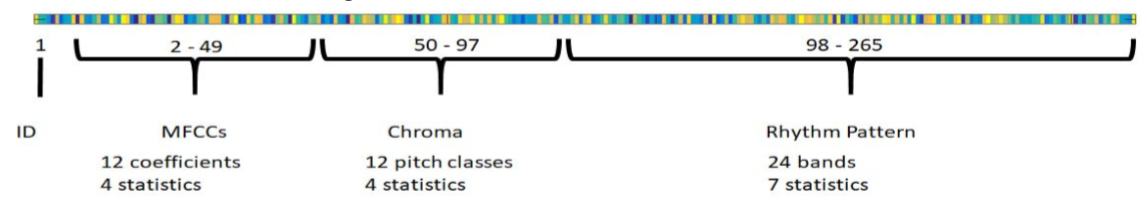
\includegraphics[width=200pt]{1_ExampleVectorStructure.PNG}
	\caption{Layout of Example Vector}
	\label{fig: Fig.1}
\end{center}
\end{figure}

\begin{figure}[h!]
The feature vector for each song thus consists of 12 coefficients representing MFFCs (using 4 statistics each), 12 pitch classes representing Chroma (using 4 statistics each), and 24 bands representing Rythm Patterns (using 7 statistics each). The details on the structure of each component of the example vector is as below: \par
\begin{center}
	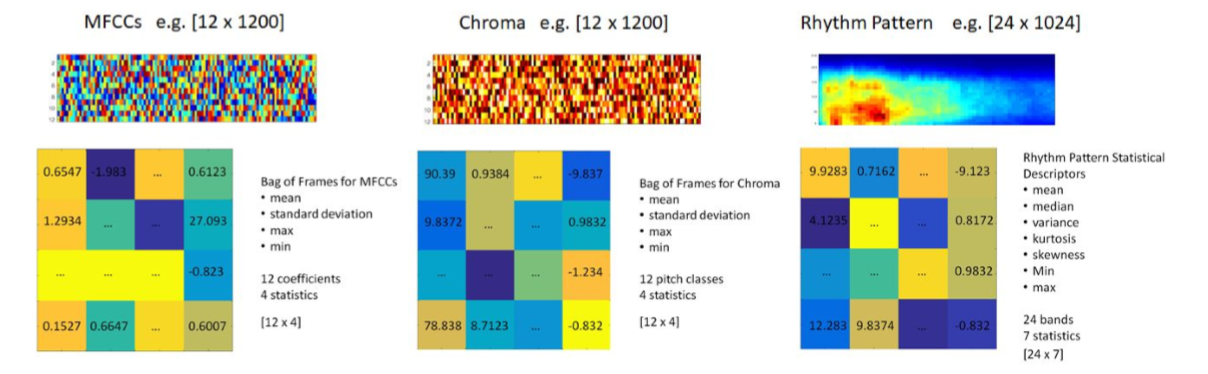
\includegraphics[width=200pt]{1_ExampleVectorStructure_2.PNG}
	\caption{Structural Representation of Example Vector}
	\label{fig:Fig.2}
\end{center}
\end{figure}

It was evident that the example features have high dimensionality, so it was decided to test an unsupervised learning approach to select create a lower dimensional dataset out of the existing dataset, to \textbf{potentially} improve performance and eliminate redundancy in the dataset. The approach adopted for this was \textbf{low dimensional embedding} [insert reference]. \par

\section{Methods and experiments}
Multiclass classification problem was explored using two different methods: \par
\begin{itemize}
	\item Low dimensional embedding with KNN clustering
	\item Multinomial logistic regression
	\item One-vs-All (OvA or OVR)
\end{itemize}
\textbf{Low dimensional embedding with KNN clustering} approach was adopted first to see if it was at all possible to reduce the high dimensions, so that the performance and accuracy issues normally associated with them could be sidestepped.\par

Low dimensional embedding employs Principal Component Analysis [insert reference] to extract useful features out of the high-dimensional dataset, essentially projecting the features to a lower dimensional space. Next, it applies K-NN clustering on the low-dimensional dataset, to prevent the ML algorithm from succumbing to the curse of dimensionality [insert reference]. \par

In our approach, we first reduced the dimensions of both our training and test datasets using PCA, followed by the application of the K-NN algorithm to acquire a model that fits our samples to appropriate labels. This model was then applied to the training and test sets, and the accuracy for both applications measured. \par

Multinomial Logistic Regression is the linear regression analysis technique used when the dependent variable is nominal with more than two levels. Thus it is an extension of logistic regression, which analyzes dichotomous (binary) dependents. Standard linear regression requires the dependent variable to be of continuous-level (interval or ratio) scale.  Logistic regression jumps the gap by assuming that the dependent variable is a stochastic event.  And the dependent variable describes the outcome of this stochastic event with a density function (a function of cumulated probabilities ranging from 0 to 1).\par
The idea is to construct a linear predictor function that constructs a score from a set of weights that are linearly combined with the explanatory variables (features) of a given observation using a dot product: \par
\begin{equation}
	score(X_i,k) = \beta_k . X_i,
\end{equation}
where $X_i$ is the vector of explanatory variables describing observation i, $\beta_k$ is a vector of weights (or regression coefficients) corresponding to outcome k, and $score(X_i, k)$ is the score associated with assigning observation i to category k. \par
In the multinomial logit model, for K possible outcomes, K-1 independent binary logistic regression models are run, in which one outcome is chosen as a "pivot" and then the other K-1 outcomes are separately regressed against the pivot outcome. \par
Therefore, for each posssible outcome, we can write down that: \par

\begin{equation}
	Equations to be inserted from wiki
	%P(Y_i = 1) = \frac{e^{\beta_1.X_i}{4}
	%\dfrac{num}{den}
	%1+ \sum_{k=1}^{K-1}e^{\beta_k.X_i}
\end{equation}

\begin{equation}
score(X_i,k) = \beta_k . X_i,
\end{equation}

\begin{equation}
score(X_i,k) = \beta_k . X_i,
\end{equation}


we can write down the expressions to for k classes as: \par
\begin{equation}
P(Y_i = 1) = 
\end{equation}



The core algorithm of the project relies on Multinomial Logistic Regression is the linear regression analysis to conduct when the dependent variable is nominal with more than two levels.  Thus it is an extension of logistic regression, which analyzes dichotomous (binary) dependents.  Since the SPSS output of the analysis is somewhat different to the logistic regression’s output, multinomial regression is sometimes used instead. \par

The second approach explored for this project was One-vs-All (also called One-vs-Rest) Classification. We train one classifier for every class, taking the samples for that particular class as positive, while the remaining samples are treated as negative. \par
The base classifer must yield a real-valued confidence score for the decision, as opposed to merely a class label, since discrete class labels could become ambiguous if results from multiple classifiers yield different labels for the same sample. \par

An algorithm describing the procedure is as follows:
\begin{itemize}
\item\textit{Inputs to the algorithm:}
\begin{itemize}
\item dataset of samples $X$ and labels $y$, where $y_{i} \in \{1, 2, ..., N\}$ is the label for the particular sample $X_{i}$
\item $L$, a binary classification training algorithm 
\end{itemize}
\item\textit{Outputs of the algorithm:}
\begin{itemize}
\item a set of classifiers $c_{n}$ for $n \in \{1, 2, ..., N\}$
\end{itemize}
\item\textit{Mechanism:}
\begin{itemize}
\item For every $n \in \{1, 2, ..., N\}$
	\begin{itemize}
	\item Build a separate label vector $z$, with $z_{i} = 1$ if $y_{i} = n$ and $z_{i} = 0$ for all other $y_{i}$
	\item Apply training algorithm $L$ on samples $X$ and label vector $z$, to get $c_{n}$ 
	\end{itemize}
\end{itemize}
\end{itemize}\par
Concretely deciding which class an unseen sample $x$ belongs to requires the application of all the obtained classifiers $c_{n}$ to it, and then choosing the label $n$ whose classifier yields the largest confidence score:
\begin{center}
${\hat{y}} =\underset{n\in\{1, 2, ..., N\}}{argmax} c_{n}(x)$
\end{center} \par
Two potential issues with the OVR are approach are:
\begin{itemize}
\item The confidence values can be different in terms of scale between each binary classifier
\item Despite the training set having a balanced class distribution, the binary classifiers will see it as unbalanced since the number of negative labels will (most likely) be much greater than the number of positive labels.
\end{itemize}
In our implementation of the OVR approach, we modify the multinomial logistic regression algorithm to generate $N$ separate classifiers. The final label for each is decided based on the classifier that results in the best confidence score.

\section{Results}

\textbf{FOR ACCURACY :}
Entry No. 1 Using multinomial :
Test Result : 
Train Result:
Result on Kaggle:

Entry No.2 Using mutinomial:
Test Result:
Train Result:
Result on Kaggle:

Test No. 3 Using OVR :
Train Accuracy : 0.7753
Test Accuracy : 0.646294881589
Result on Kaggle : 0.62882 (Improvement)

\textbf{FOR LOG-LOSS}
Entry No. 1:
2.60627 (using multinomial)



\section{Conclusion}
\blindtext

\section{Appendices}
\blindtext
\begin{appendices}
	\chapter{Some Appendix}
	The contents...
\end{appendices}


\section{Proof of the First Zonklar Equation}
Some text for the appendix.
% use section* for acknowledgement
\section*{Acknowledgment}


The authors would like to thank...


% Can use something like this to put references on a page
% by themselves when using endfloat and the captionsoff option.
\ifCLASSOPTIONcaptionsoff
  \newpage
\fi




% references section

% can use a bibliography generated by BibTeX as a .bbl file
% BibTeX documentation can be easily obtained at:
% http://www.ctan.org/tex-archive/biblio/bibtex/contrib/doc/
% The IEEEtran BibTeX style support page is at:
% http://www.michaelshell.org/tex/ieeetran/bibtex/
%\bibliographystyle{IEEEtran}
% argument is your BibTeX string definitions and bibliography database(s)
%\bibliography{IEEEabrv,../bib/paper}
%
% <OR> manually copy in the resultant .bbl file
% set second argument of \begin to the number of references
% (used to reserve space for the reference number labels box)
\begin{thebibliography}{1}
%\bibitem{Million_Songs}	
%	title  = "Million Song Dataset | scaling MIR research",
%	url    = "https://labrosa.ee.columbia.edu/millionsong/",% Ref : https://engineering.purdue.edu/~mark/puthesis/faq/cite-url/
%\bibitem{PCA_definiation}
%	title = ''Using PCA for Dimensionality Reduction''
%	url = ''https://www.analyticsvidhya.com/blog/2015/07/dimension-reduction-methods/ ''
	
\end{thebibliography}


% biography section
% 
% If you have an EPS/PDF photo (graphicx package needed) extra braces are
% needed around the contents of the optional argument to biography to prevent
% the LaTeX parser from getting confused when it sees the complicated
% \includegraphics command within an optional argument. (You could create
% your own custom macro containing the \includegraphics command to make things
% simpler here.)
%\begin{biography}[{\includegraphics[width=1in,height=1.25in,clip,keepaspectratio]{mshell}}]{Michael Shell}
% or if you just want to reserve a space for a photo:

%\begin{IEEEbiography}{2}
%Article title:	Million Song Dataset | scaling MIR research
%Website title:	Labrosa.ee.columbia.edu
%URL:	https://labrosa.ee.columbia.edu/millionsong/
%\end{IEEEbiography}
% You can push biographies down or up by placing
% a \vfill before or after them. The appropriate
% use of \vfill depends on what kind of text is
% on the last page and whether or not the columns
% are being equalized.

%\vfill

% Can be used to pull up biographies so that the bottom of the last one
% is flush with the other column.
%\enlargethispage{-5in}



% that's all folks
\end{document}


